\section{Experiments}
\subsection{Optimal solution verification}
In all cases, interface code was written so that the original author's code could be run without modification. Two methods were used to verify solution correctness: 1. manual visual verification of results for approximately 100 random graph pairs and 2. solution size verification against a second algorithm. The first method is used primarily as a sanity check on code integration. An example of the output MCS solution is below. 

\TODO{insert sample image of highlighted MCS mappings}

The second method follows the rationale that if multiple "optimal" search algorithms agree, then the algorithms are likely to be correct \cite{korf2014you}. We verify these results by using a second algorithm \cite{mccreesh2016clique} to solve the same MCS problem and compare the solution sizes. It should be noted that these algorithms output a single optimal mapping. As a result, while the mappings may differ between algorithms, we verify correctness using the MCS size. We use the author's original implementation and verified that for all three datasets (AIDS, LINUX, and IMDB), that the two solutions sizes are consistent.

\subsection{Baseline output stats}
Since we would like to train a network to predict the MCS of two graphs, we need to quantify the limits of the current state of the art algorithms. Following existing methods to quantify solution speed \cite{hoffmann2018observations}, we look at the percentage of MCS graph pairs that can be optimally solved in a given time limit, as a function of pairwise graph size, as shown in Figure \ref{fig:solution_limits}. The pairwise graph size metric used is the minimum number of nodes in either graph of the graph pair. For small graphs (the AIDS and LINUX datasets), the McSpilt algorithm solves all instances in less than 1 second. Therefore, we analyze the IMDB dataset, setting a time limit of 1 minute for every solution.

\begin{figure}
    \center
    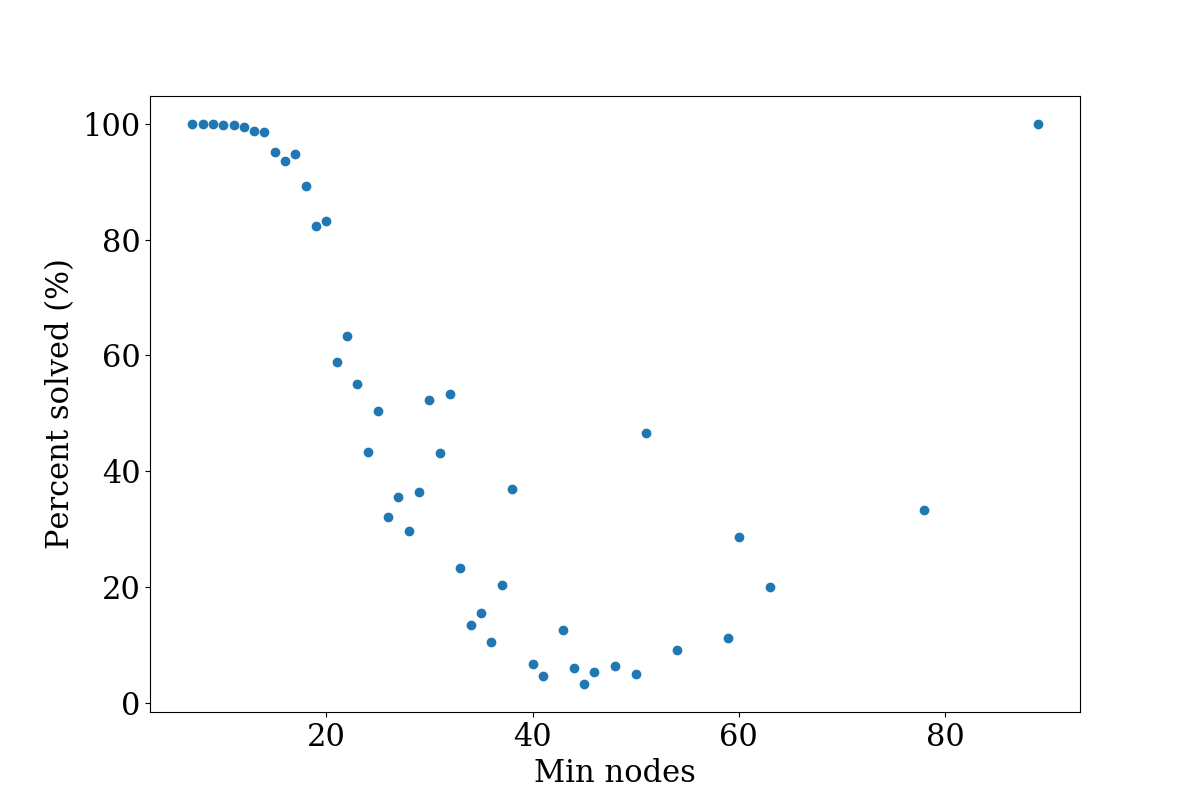
\includegraphics[width=0.8\textwidth]{figures/pct_solved_avg_nodes.png}
    \caption{Percent of MCS pairs from the IMDB dataset solved for a given pairwise graph size with a 1 minute time limit. Pairwise graph size metric is the minimum number of nodes contained in either graph.}
    \label{fig:solution_limits}
\end{figure}

As expected, there is a general downwards trend of percent of pairs solved for increasing graph size. Although there exists significant noise in the solved percentage, it appears that the exact algorithm fails to solve 50\% of the cases for graph pair size of approximately 20 nodes and more than 90\% of the cases for sizes greater than 40 nodes.

The noisiness in the data exists due to the dataset analyzed. Some input graphs are easy for the exact solver, and since the dataset has a limited number of large graphs, easy solutions skew the data towards 100\%. This is particularly noticeable for graph size = 89, in which all pairs were solved for that graph size. IMDB contains only 1 graph of size 89 which happens to have this quality, so all solution pairs involving that graph are solved.

\subsection{Trained AAAI model and results}
Following the results in \cite{bai2018convolutional}, we train a model on the task of similarity search, where the similarity metric is the nMCS. We use mean squared error (mse), Kendall's Rank Correlation Coefficient $\tau$ \cite{kendall1938new}, Spearman's Rank Correlation Coefficient $\rho$ \cite{spearman1904proof}, and Precision at k (p@k) to evaluate the model. It should be noted that rather than develop a new model to specifically learn the MCS problem, this work is focused on showing that MCS is a reasonable metric for similarity search and is learnable with an existing state-of-the-art model.


\begin{table}
% AIDS.
  \center
  \caption{Results on AIDS}
  \label{table:aids}
\begin{tabular}{|c|P{1.6cm}|P{1.6cm}|P{1.6cm}|P{1.6cm}|P{1.6cm}|}

\hline
 & $\mathrm{mse}(10^{-3})$ & $\rho$ & $\tau$ & p@10 & p@20 \\
\hline
GSimCNN (GED) & 3.16 & 0.84 &  & 1 & \\
\hline
GSimCNN (MCS) &  &  &  &  & \\
\hline
\end{tabular}

\bigskip

% LINUX.
  \center
  \caption{Results on LINUX}
  \label{table:linux}
\begin{tabular}{|c|c|c|c|c|c|}

\hline
 & $\mathrm{mse}(10^{-3})$ & $\rho$ & $\tau$ & p@10 & p@20 \\
\hline
GSimCNN (GED) &  &  &  &  & \\
\hline
GSimCNN (MCS) &  &  &  &  & \\
\hline
\end{tabular}
\end{table}

- include the standard plot results

- include some sample ranking results

